\section*{Assignment 03: Evolution of the Platform Concept}
\addcontentsline{toc}{section}{Assignment 03: Evolution of the Platform Concept}

\subsection*{Why the pivot happened}
My earliest sketches centrd on a \textbf{dinner experience marketplace}. Applying \citet{Choudary2016}'s \textit{asset light checklist} exposed two conflicts: the concept required controlling physical spaces and guaranteeing food safety, which would turn the platform into an \textbf{operator} rather than an \textbf{orchestrator}. Lecture~6 also highlighted how platforms that ignore regulatory friction didn't understand the \textbf{winner takes all} dynamics \citep{Lecture06}. Combining those lessons with \citet{Srnicek2017}'s critique of extractive gig models convinced me to \underline{stop} investing energy there.

\subsection*{Using the platform design toolkit in practice}
When the SkillSync idea came to life, I worked through the entire \citet{Reillier2017} toolkit rather than referencing it abstractly. Table~\ref{tab:platform-map} documents this. The toolkit prompts six questions: who are the \textbf{producers}, who are the \textbf{consumers}, what is \textbf{the core value} unit, which \textbf{partners support the interaction}, what \textbf{governance rules} apply at each step, and how do we \textbf{measure success}. Students act as producers, NGOs as consumers, mentors as partners, and the value unit is a matched with a project response. Governance rules include email verification, a simple process, mentor escalation, and dispute templates. Success metrics focus on completion rate, satisfaction, and repeat participation. Writing these answers forced me to operationalise the interaction and now doubles as a onboarding checklist.

\begin{table}[H]
  \centering
  \caption{Platform design toolkit worksheet filled for SkillSync based on \citet{Reillier2017}.}
  \label{tab:platform-map}
  \begin{tabular}{p{0.22\linewidth}p{0.33\linewidth}p{0.33\linewidth}}
    \toprule
    Role & Value created and exchanged & Governance guardrail \\
    \midrule
    Students & Verified skill profiles, availability windows, project reflections & Institutional email check, mentor references, code of conduct signoff before browsing briefs \\
    Organisations & Scoped briefs with deliverables, support statements, impact metrics & Wizard enforces clarity on scope, timeline, support, and evaluation criteria before publishing \\
    Mentors and faculty & Feedback comments, escalation paths, reference letters & Moderation rights and retrospectives that log concerns within twenty four hours \\
    Platform team & Matching algorithm, stipend disbursement, analytics dashboards & Data minimisation, opt in analytics reviews, and audit trail reviewed in Assignment~05 \\
    \bottomrule
  \end{tabular}
\end{table}

After the toolkit pass, i prototyped the organisation process in Figma and prepared \textit{hallway testing} with two NGOs from previous courses. The script asked them to fill the template while thinking out load; the focus was to see whether the prompts prevented creep without sounding bureaucratic. Notes from those sessions directly informed Figure~\ref{fig:project-creation}.

\subsection*{Rituals that kept the change grounded}
Avoiding to pivot, I documented every experiment. Each time I scored candidate moves against \textit{desirability}, \textit{feasibility}, and \textit{viability} using a simple 1-5 rubric. If a score dropped below 3 I paused the idea. For example, the dinner marketplace lost feasibility points because health compliance looked expensive, while SkillSync gained desirability thanks to campus access. I also ran a rehearsal: pairing one NGO brief with two student teams manually to test the workflow. The exercise confirmed that the checklist reduced confusion, so I kept investing in the SkillSync route. These rituals follow \citet{Choudary2016}'s guidance on \textit{iterative governance and echo} Lecture~6's insistence that pivots should be \textbf{theory informed rather than impulsive} \citep{Lecture06}.

Figure~\ref{fig:project-creation} shows the final process draft. Each section corresponds to a governance lever from \citet{Reillier2017}: define the value unit, specify contributions, and clarify rewards. Helper text explains why each field matters so organisations feel coached instead of interrogated.

\begin{figure}[H]
  \centering
  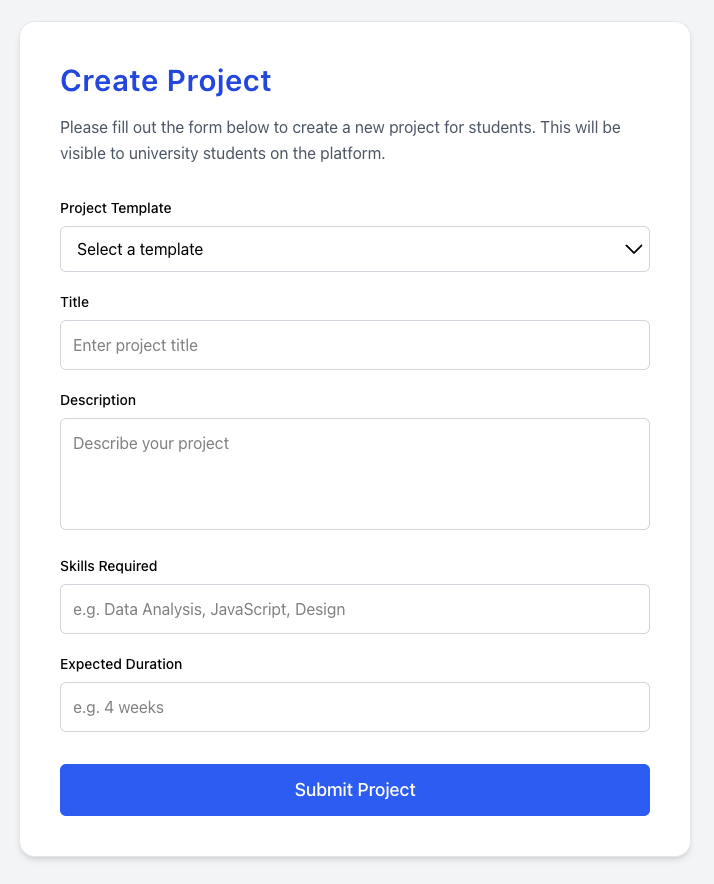
\includegraphics[width=0.85\linewidth]{figures/Organisation-generate-project.png}
  \caption{Organisation project wizard mock up that operationalises the toolkit entries.}
  \label{fig:project-creation}
\end{figure}
